% !TEX root = ../../prj4projektrapport.tex
% SKAL STÅ I TOPPEN AF ALLE FILER FOR AT MASTER-filen KOMPILERES 

\section{Test}

I dette afsnit vil der ikke blive gået i dybden med de enkelte tests, men derimod selve testprocessen og tankerne gjort i testfasen. For at se mere om de enkelte udførte test, se dokumentationen\footnote{Projektdokumentation, 10.4, Modultest}.

Da Styringsenheden generelt har indeholdt meget programmering, har det været oplagt at teste funktionaliteten af koden på andre allerede udviklede moduler i projektet.  Eksempelvis er funktionaliteten af Brugergrænsefladen testet med brug af andre allerede testede moduler. Til testen af Brugergrænsefladen er kommunikationen fra Måleenhed til Kommunikationsmodul og videre til Kontrolmodulet brugt for at genere tilfældige data, der så blev sendt og udskrevet på HMI'en fra Kontrolmodul. Det samme gælder testen af kommunikationsoprettelsen udført af PLC'en, her er benyttet en PC med et testprogram, der bruges til at udskrive information om TCP kommunikationen. Det har ved brug af dette testprogram været muligt at indsætte debug udskrifter og på den måde følge forbindelsen efter og tilbage, samt se hvor der var eventuelle fejl.  Herunder ses et enkelt testeksempel, hvor dette test program har været benyttet, se figur \ref{fig:TestModtagSendData}. For hele testbeskrivelsen refereres til dokumentationen\footnote{Projektdokumentation, 10.4.1, Kontrolmodul}.


\begin{figure}[H] % (alternativt [H])
	\centering
	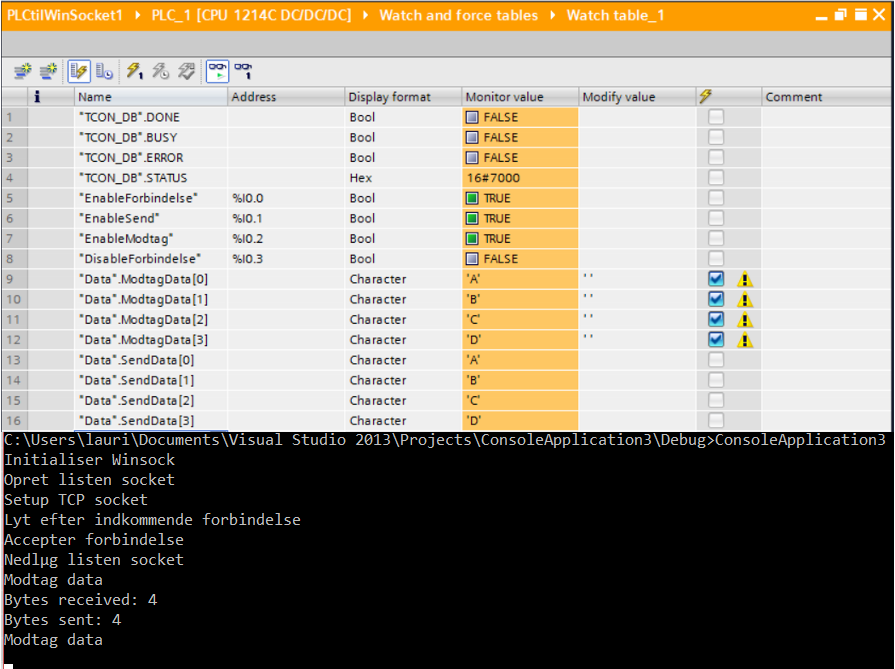
\includegraphics[width=0.85\textwidth]{figure/ModtagDataOgSendData}
	\caption{Test af ModtagData og SendData}
	\label{fig:TestModtagSendData}
\end{figure}
